\chapter{Supervaluationism, Dynamic Supervaluationism, and Higher-Order Vagueness}
\chaptermark{Supervaluationism, Dynamic Supervaluationism, and Higher-Order Vagueness}
\chapterauthor{Wiktor Przybrorowski, \textit{
University of St Andrews
}}
\renewcommand*{\thesection}{\arabic{section}.}
\renewcommand*{\thesubsection}{\arabic{section}.\arabic{subsection}.}

\begin{quote}
The fact that the phenomenon of vagueness can itself be vague---and 
its vagueness be vague as well---seems impossible to make sense of
without getting a headache. This so--called higher--order vagueness makes
theorising about vagueness a notoriously difficult task for philosophers
of logic and language. This difficulty manifests itself in that, even if
a theory can convincingly explain what vagueness is and how we can
reason about it, when faced with the vagueness of the just--tamed
vagueness, it gets flooded with paradoxes and makes the initial theory
seem implausible. In this paper, I argue that Rosanna Keefe's
supervaluationism is one such theory. Even though it elegantly accounts
for the first order of vagueness, it becomes less elegant when
questioned about the higher orders. To demonstrate this, I show that
Keefe's system fails to resolve various paradoxes of higher-order
vagueness such as the finite series paradox or the $D^*$ paradox.
Furthermore, I argue that in her attempts to accommodate the paradoxes
by adopting a rigid hierarchy of metalanguages, Keefe invites new
worries. Given these criticisms, it is unlikely that Keefe's theory can
be `argued out' of these paradoxes---`finite series' in particular.
Instead, I argue that the theory must be substantially modified if it is
to be salvaged, and one way to do so is by making the proposed structure
more dynamic. I attempt to do so by sketching an outline of dynamic
supervaluationism that can tackle the problems that Keefe's
supervaluationism cannot. I close my essay by teasing out some
challenges that the proposed theory could face and offering possible
solutions. I believe that supervaluationism is a very attractive
approach to vagueness and therefore, it is worth developing further into
a more robust theory that could tackle its higher orders.
\end{quote}

\section{Introduction}

Vagueness in language refers to an indeterminate relationship between
its terms and the world they describe.\footnote{Kit Fine,
  \emph{Vagueness: A Global Approach} (Oxford Academic, 2020), 2-3.} Minimally,
a predicate is vague if it has three features: \textbf{admission of
borderline cases} (objects to which its application is unclear),
\textbf{a lack of known, sharp boundaries} (no clear case separating the
positive and negative cases), and (apparent) \textbf{susceptibility to
the Sorites paradox}.\footnote{Rosanna Keefe, \emph{Theories of
  Vagueness}, (Cambridge University Press, 2000), 6-7.}

Vagueness is philosophically relevant because it raises two problems.
First, the \textbf{semantic problem}: since the vague extension is
unclear, classical semantics (where meaning is derived from extension),
and hence classical logic, may not apply. Second, the \textbf{Soritical
problem}. Consider a series of people of descending heights by 1cm. The
first is clearly tall (200cm) and the last is clearly not (120cm). Since
no known boundaries exist, vague predicates are tolerant---a small
change will not alter the application. Thus, by inductive step, for any
case $\mathbf{n}$, `if $\mathbf{n}$ is tall then $\mathbf{n}+1$ is tall'.
Starting at 200cm is tall, via a series of conditionals, you validly
conclude that 120cm is tall. However, this is a contradiction since
120cm is clearly not tall.\footnote{Fine, \emph{Vagueness}, 3-7.} This
argument exemplifies the classical form of the Sorites paradox.

Theorizing about vagueness involves accounting for the nature, source
and meaning of vagueness, providing vague semantics and resolving the
Sorites. Furthermore, since it is unknowable where the positive
extension changes to negative, it is equally unknowable where the
positive changes to borderline. Thus, borderline cases themselves should
be unbounded; hence there should be borderlines to borderlines. The
process could be iterated to establish a possibly infinite hierarchy of
borderline cases: the higher--order vagueness (HOV).\footnote{Keefe,
  \emph{Theories of Vagueness}, 31-32.}

Throughout this paper, I will follow Rosanna Keefe and other major
supervaluationists in assuming that HOV is a genuine problem, that needs
to be accounted for. However, it is worth pointing out that this is a
debated matter in the field.\footnote{Some philosophers, such as Dominic
  Hyde, claim that higher--order vagueness (HOV) is a pseudo--problem,
  arguing that the vagueness of vague is a real, but unproblematic,
  phenomenon. Others, including Hao--Cheng Fu and Susanne Bobzien counter
  that this stance fails to adequately address the complexity of the
  issue, maintaining that HOV is indeed a genuine problem. While an
  extensive discussion is beyond the scope of this essay, see Hyde, "Why
  Higher--Order Vagueness Is a Pseudo-Problem"; Fu, "Saving
  Supervaluationism from the Challenge of Higher-Order Vagueness
  Argument''; and Bobzien, "In Defense of True Higher-Order Vagueness"
  for further details.} Nevertheless, under this assumption a successful
theory of vagueness, given its commitments, must also account for HOV.

In this essay, I explore how one theory of vagueness---supervaluationism, advocated by Rosanna Keefe---does so. First, I
outline her account of first--order vagueness (FOV). Then, I explain the
problems posed by HOV, examining Tim Williamson's criticisms of the
theory and how Keefe accommodates them. I will argue that although the
Williamson problems are solved, the resulting view does not reflect how
language actually functions and is paradoxical, making the HOV account
unsatisfactory. I then attempt to modify the view by dynamizing it,
developing the ideas of Hao--Cheng Fu. I defend the model by showing how
it solves some of the critical issues faced by Keefe. Lastly, I raise a
few possible issues endemic to the dynamic view and sketch responses to
defend it.

\section{Supervaluationism, a theory of vagueness}

Supervaluationists claim that vagueness is a problem of language, not
our epistemic capacities. They argue that vague predicates fail to draw
sharp boundaries, not that these boundaries are unknowable, and that
they admit borderline cases. The source is semantic indecision. A vague
predicate admits a range of possible extensions, but it is semantically
unsettled which one is correct. This is captured through the notion of
precisification, a way to make a vague term precise.\footnote{Keefe,
  \emph{Theories of Vagueness}, 154-156.} A precisification must be
admissible, reasonable in not licensing a misuse of language.\footnote{Timothy
  Williamson, \emph{Vagueness}, (Routledge, 1994), 158.} It also must be
complete, it categorizes objects into positive and negative extensions,
leaving nothing in--between. For illustration, consider the vague
predicate `tall'. We could (reasonably) use precisifications: `tall' is
true if `\textgreater175cm', `\textgreater180cm' and
`\textgreater190cm', each of which would precisely divide objects into
positive and negative extensions. Vague terms do not `choose' between
these; instead, all precisifications are equally good.\footnote{Keefe,
  \emph{Theories of Vagueness}, 154-156.}

Supervaluationists provide semantics for vague predicates, identifying
truth with super--truth by considering all possible precisifications.
$F\mathbf{a}$ is super--true (-false) iff $F$ is true (false) of
$\mathbf{a}$ under all complete and admissible precisifications.
$F\mathbf{a}$ is neither true nor false iff $F$ is true of
$\mathbf{a}$ under some precisifications and false of $\mathbf{a}$ under
others.\footnote{Keefe, \emph{Theories of Vagueness}, 154.}

Thus, vague predicates divide objects in a three--fold manner, where
borderline cases are not assigned a definite truth value. Hence,
supervaluationists give up bivalence, departing from classical
semantics, by admitting truth value gaps. On the other hand, classical
logic is mostly preserved because if a sentence is classically true,
then it is true on all complete and admissible precisifications.
Consider the law of excluded middle. Using any precisification of tall---every object will be either tall or not-tall, since every
precisification divides objects into two sharp sets. Similarly, all
classical theorems are retained, thus we can use classical logic to
reason about vague predicates.\footnote{Rosanna Keefe, ``Vagueness:
  Supervaluationism,'' \emph{Philosophy Compass} 3, no. 2 (2008):
  162-164.}

This idea provides a straightforward solution to the Sorites. Namely,
the inductive premise `if $F\mathbf{n}$ then $F(\mathbf{n}+1)$' is
super--false, since the antecedent will be true and the consequent false
for some $\mathbf{n}$ under any complete and admissible precisification.
This is because each precisification, being complete, provides a sharp
cut--off between the true and false---a bordering pair where the first
entry is true and second one is false.\footnote{Keefe, ``Vagueness:
  Supervaluationism,'' 315-316.} Thus, the supervaluationist account
fulfils the initial demands of theorizing about vagueness. Consult the
footnote\footnote{Consider the series of people of varying heights again
  and suppose some examples of complete precisifications: $\mathbf{x}$ is
  short if (1) `$<160\text{cm}$' or (2) `$<165\text{cm}$' or (3)
  `$<170\text{cm}$'. They are complete since they divide objects into
  positive (short) and negative (not--short) extensions with nothing
  in-between. It is easy to see how the inductive premise turns out
  false on each of these precisifications: (1) `If 159cm is short, then
  160 is short'; (2) `If 164cm is short, then 165cm is short'; (3) `If
  169cm is short, then 170cm is short'. In each case, the antecedent is
  true and the consequent false (relative to precisification). Since the
  inductive premise turns out false for some pair under each complete
  precisification, it is super-false.} for further clarification.

\section{Supervaluationism and higher-order vagueness}

The above metalanguage (talk of truth conditions) expresses the
vagueness of the object language by dividing cases into three sharply
bounded sets (true, false, borderline). This can be captured by adding a
`definitely' $D$ operator to the object language, which functions akin to
modal necessity.

The FOV of $F$ is expressed as:

\begin{enumerate}
\def\labelenumi{(\arabic{enumi})}
\item
  $DFx$ for definite positive cases (true under all complete and
  admissible precisifications)
\item
  ${\sim} DFx \, \& \, {\sim} D {\sim} Fx$ for borderline cases (true/false
  under some)
\item
  $D {\sim} Fx$ for negative cases (false under all)
\end{enumerate}

This division is problematic since all cases are sharply categorized,
allowing no borderlines between the definite and borderline cases,
leaving no scope for HOV. Supervaluationists argue that this can be
resolved by allowing the concept of `admissibility' itself to be vague,
thus making the metalanguage vague.\footnote{Keefe, \emph{Theories of
  Vagueness}, 202-204.}

Hence, the second--order vagueness of $F$ is captured in the
meta--metalanguage by expressing vagueness of $DF$ (the metalanguage). This
yields the following five--fold classification:

\begin{enumerate}
\def\labelenumi{(\arabic{enumi})}
\item
  $DDFx$, i.e., definitely definitely positive cases
\item
  ${\sim} DDFx \; \& \; {\sim} D {\sim} DFx$, i.e., borderline between positive
  and borderline
\item
  $D {\sim} DFx \; \& \; D{\sim} D{\sim} Fx$, i.e., definitely borderline cases
\item
  ${\sim}DD{\sim} Fx \; \& \; {\sim}D{\sim}D{\sim}Fx$, i.e., borderline between
  negative and borderline
\item
  $DD{\sim}Fx$, i.e., definitely definitely negative cases
\end{enumerate}

The general idea is that for  level vagueness of F, we need
to show that $\mathbf{n}$ categories are vague. Thus, we need borderlines
between those, in effect, drawing $2^n+1$ categories.\footnote{Mark
  Sainsbury, ``Concepts without Boundaries,'' in \emph{Departing From
  Frege} (Routledge, 1990), 74.}

\subsection{Williamson's challenge}

Williamson argues that for this formalization to work, the D operator
should not obey these two schemas:
\begin{enumerate}
\def\labelenumi{(\arabic{enumi})}
\item{The S5 principle: If ${\sim}DF$, then $D{\sim}DF$.}
\item{The S4 principle: If $DF$, then $DDF$.}
\end{enumerate}

If (1) and (2) hold, then whether a category is definite or indefinite,
it will also be definitely so at higher levels. The supervaluationist
cannot accept this since each category must be vague, otherwise it would
draw sharp boundaries. Thus, Williamson recommends adopting a weaker
modal logic, like T, with relative admissibility and no transitivity so
that both S4 and S5 principles fail.\footnote{Williamson,
  \emph{Vagueness}, 156-159.} See the appendix for a more formal
explanation.

However, Williamson argues that this is not sufficient to solve the
problem via the $D^*$ argument. He defines $D^*\hspace{-0.2em}F$ as an infinite
conjunction $F \ \&  \ DF \ \& \ DDF \ \& \ldots \& \ D_{n}F$. Suppose
precisifications (a), (b), and (c), where (a) admits (b), and (b) admits
(c), but (a) does not admit (c), since admissibility is non-transitive.
Suppose $D^*\hspace{-0.2em}F$ at (a). This means that
$F, \ DF, \ DDF, \ \ldots, \ D_{n}F$ are true at (a). If $DF$ is true at
(a), then $F$ is true at (b); if $DDF$ is true at (a), then $DF$
is true at (b); and so on. Thus, $F, \ DF, \ DDF, \ \ldots, \ D_{n}F$ are
all true at (b), and hence $D^*\hspace{-0.2em}F$ is true at (b). The same reasoning
applies to (c). Thus, if $D^*\hspace{-0.2em}F$ is true at some precisification,
then $D^*\hspace{-0.2em}F$ is true at all precisifications. Hence, ${DD}^{*}F$ is
true at all precisifications---and by the same reasoning, so is
$D^*\hspace{-0.2em}D^*\hspace{-0.2em}F$. Therefore, the S4 principle effectively applies to
$D^*$ (see diagram below).

\begin{center}
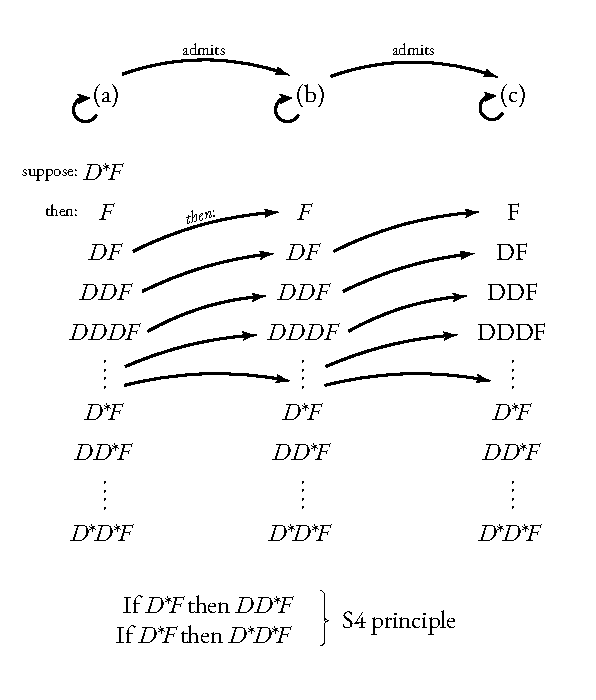
\includegraphics[width=3.97674in,height=4.66543in]{papers/figures/2-1.pdf}
\end{center}
Consequently, Williamson concludes that higher--order vagueness
disappears.\footnote{Williamson, \emph{Vagueness}, 160.} This is
because, for supervaluationism to succeed, each metalanguage must be
vague. Thus, supervaluationists need a borderline case between
$D^*\hspace{-0.2em}F$ and $D^*{\sim}F$, namely
${\sim}DD^*\hspace{-0.2em}F \ \& \ {\sim}D{\sim}D^*\hspace{-0.2em}F$. However, ${\sim}DD^*\hspace{-0.2em}F$
collapses to ${{\sim}D}^{*}F$ by modus tollens on the S4 principle. ${\sim}D^*\hspace{-0.2em}F$ then collapses to $D {\sim}D^*\hspace{-0.2em}F$, given closure of
D.\footnote{Patrick Greenough, ``Higher-Order Vagueness,''
  \emph{Proceedings of the Aristotelian Society, Supplementary Volumes}
  79 (2005): 183.}
In effect, ${\sim}DD^*\hspace{-0.2em}F \ \& \ {\sim}D{\sim}D^*\hspace{-0.2em}F$ reduces to $D{\sim}D^*\hspace{-0.2em}F \ \& \ {\sim}D{\sim}D^*\hspace{-0.2em}F$ which is a contradiction.
Since there are no borderlines to $D^*\hspace{-0.2em}F$, it is not vague.

Williamson offers supervaluationists a way out: to give up semantic
closure. $D^*$ can be vague but its vagueness cannot be expressed using $D$
or $D^*$. Instead, we need a meta--language for $D^*$, enriched with a distinct
operator, $D!$. Then, to express vagueness of $D!$, we need a
meta--metalanguage with $D!!$. Williamson remarks that the process could
continue infinitely.\footnote{Williamson, \emph{Vagueness}, 160-161.}

Keefe takes up this proposal and advocates adopting an infinite,
hierarchical series of metalanguages. In this model, the vagueness of
the $n^{\text{th}}$-level metalanguage can only be expressed in the $(n+1)^{\text{th}}$
metalanguage, which is essentially richer than the nth language. She
argues that, since there is no reason not to adopt such an infinite
sequence, she can just stipulate that all the languages in the series
are vague.\footnote{Keefe, \emph{Theories of Vagueness}, 202-208.}
Greenough sketches a formalization where the object language is enriched
with indexed D operators where each \(D_{n + 1}\) is used to express the
vagueness of \(D_{n}\). Such formalization stops the $D^*$ paradox and
ensures that a non-vague metalanguage cannot be generated.\footnote{Greenough,
  ``Higher-Order Vagueness,'' 184-186.}

\section{Evaluation}

Even though the above account might seem abstract, its strength lies in
its simplicity---Keefe only iterates her account of the first order to
higher orders of vagueness. In effect, the initial solutions to
vagueness problems equally apply to HOV. Vagueness at higher orders
remains a matter of semantic indecision: we are undecided over whether a
precisification counts as admissible. Furthermore, each level $n$
admits borderline cases and lacks sharp boundaries---a fact that can be
expressed in the $n+1$ metalanguage using appropriate D operators.

Moreover, each higher order metalanguage is still Sorites susceptible. I
will explain this by running the paradox for the metalanguage (second
order vagueness) in natural language terms for clarity---though the same
could be done using D operators. The inductive premise for the
metalanguage can be restated, in natural language, as: `if there are
admissible precisifications that draw the boundary to `tall' at height
h, then there are ones that draw it at one-hundredth of an inch
lower'.\footnote{Keefe, \emph{Theories of Vagueness}, 207-208.} The
second order series could start with a clearly admissible
precisification (e.g., taller than 190cm) and end with a clearly
inadmissible one (e.g., taller than 110cm). Since one--hundredth of an
inch does not make a difference in admissibility, you could run a series
of conditionals, starting with `taller than 190cm is admissible' to
reach a conclusion that `taller than 110cm is admissible'. This is a
contradiction. To resolve the second-order paradox, Keefe reuses her
earlier strategy: for any complete way of making `admissible' precise
(or making `definitely' definite), there will be a pair such that the
first precisification is admissible and the second is not. This could be
run for any level of metalanguage.

Thus, Keefe's account of HOV fulfils all the demands of a theory of
vagueness. Each metalanguage is vague since it (1) admits borderline
cases, (2) draws no sharp boundaries and (3) is Sorites susceptible. The
fact that she achieves this for each order while maintaining her initial
commitments (using the same technique at each order, characterising all
levels of vagueness as semantic indecision, and so on) makes her
strategy simple and elegant.

Even though this iteration neatly maintains the supervaluationist
method, iterating to infinity is problematic. Keefe boldly claims that
`if there is no general objection to the claim that the sequence of
metalanguages for metalanguages is infinite, then what is the difficulty
with adding `and each of those languages is vague'\,'.\footnote{Keefe,
  \emph{Theories of Vagueness}, 208.} However, there is a fundamental
difficulty in this addition. In Keefe's system, the vagueness of an
n-level metalanguage can only be expressed via an $n+1$ level
metalanguage. If all metalanguages are vague, then the infinite
metalanguage would have to be vague. To express the vagueness of the
infinite metalanguage, we would need to use the infinity $+ 1$
metalanguage. However, adding another element to an infinite set would
not alter the size of this set.\footnote{MIT OpenCourseWare,
  \emph{Session 11: Mathematics for Computer Science}, \emph{6.042J:
  Mathematics for Computer Science, Spring 2015} (Massachusetts
  Institute of Technology, 2015).}
Thus, the infinite $+ 1$ metalanguage would be on the same meta -level as
the infinite metalanguage. Hence, the vagueness of the infinite
metalanguage cannot be expressed and the statement `each of those
languages is vague' seems meaningless.

This objection points towards a more general issue with such Tarskian
metalanguage hierarchies. Namely, that languages in such hierarchies
cannot be globally quantified over.\footnote{Greenough, ``Higher-Order
  Vagueness,'' 187.} Keefe could respond that even though the infinite
metalanguage might not be definable in her structure, it does not mean
that it does not exist. Her structure ensures that vagueness for any
finite level can be expressed. Even though we cannot say that `all
metalanguages are vague', we also cannot identify any non--vague
metalanguage within the structure. Thus, even though the concept of
infinity proves problematic for Keefe at the outset, I will assume that
this problem does not threaten the explanatory power of her structure.

A further problem with the structure is that it is highly detached from
how language functions. Competent speakers would find making sense of
iterated uses of `definitely' difficult, whether it is indexed or not.
For example, saying someone is `definitely definitely definitely tall'
has little meaning apart from emphasis. Keefe might respond by pointing
out that we do not use expressions like `a googol of a googol of a
googol' in ordinary conversation either, yet this does not mean the
concept of `googol' is not a meaningful mathematical concept. However,
the issue goes deeper. As Saul Kripke pointed out, we cannot
consistently assign levels to truth. Thus, even if we index the levels
of `definitely', it is difficult to assign them consistently. Consider
the following statements: Jan says, `Everything Alfred said is
definitely false', and Saul says, `Everything Jan said is definitely
false'. To make sense of these, we would need to place one at a higher
level in the hierarchy. However, this does not happen in natural
language.\footnote{Saul Kripke, ``Outline of a Theory of Truth,''
  \emph{The Journal of Philosophy} 72, no. 19 (1975): 694-697.}

Keefe might counter these natural language intuitions by arguing that
her model is only an idealization which is not meant to exactly
replicate how ordinary language works. While iterating `definitely'
(e.g., \(D_{3}D_{2}D_{1}F\)) may make little sense in casual
conversation, the model is primarily defended by its explanatory power
regarding HOV. She could further argue that even though different levels
of metalanguages, when expressed in natural language, might not be
clearly marked and distinguishable (such as in the Jan--Alfred example
above), they can still function as distinct metalanguages in a formal
framework. A further worry is that such an approach might over--idealise
HOV making her account arbitrary. It raises the question over whether
speakers genuinely use implicitly distinct levels of metalanguages to
assign levels to truth. Thus, Keefe would need to give a more robust
explanation of the relationship between her model and natural
language.\footnote{A full discussion of this issue is beyond the scope
  of this essay, though the problem would require further explanation to
  defend the account effectively.}

Lastly, even though Keefe's iteration method allows her to respond to
Williamson's $D^*$ paradox and establish that there cannot be a non-vague
metalanguage, the non-vagueness of each metalanguage requires further
borderline cases. We need \(2^{n} + 1\) categories to express the
vagueness of the nth metalanguage. However, there is a tension between
an infinite number of categories and a finite number of objects in the
series: the finite series paradox. Consider a simple series with 5
objects. To account for 1\textsuperscript{st} level, we divide them into
3 categories. To account for 2\textsuperscript{nd} level, we divide them
into 5 categories. At 3\textsuperscript{rd} level there are 9 categories
to be filled but only 5 objects. This means that at some level we will
run out of objects with which to fill the categories. As a result, there
will be no borderline cases between the categories - providing a sharp
boundary, as pictured below.\footnote{Greenough, ``Higher-Order
  Vagueness,'' 180; 185-186.} Whether or not Keefe indexes her D
operators makes no difference, there will always be an insufficient
number of objects in the series to fill all categories.
\begin{center}
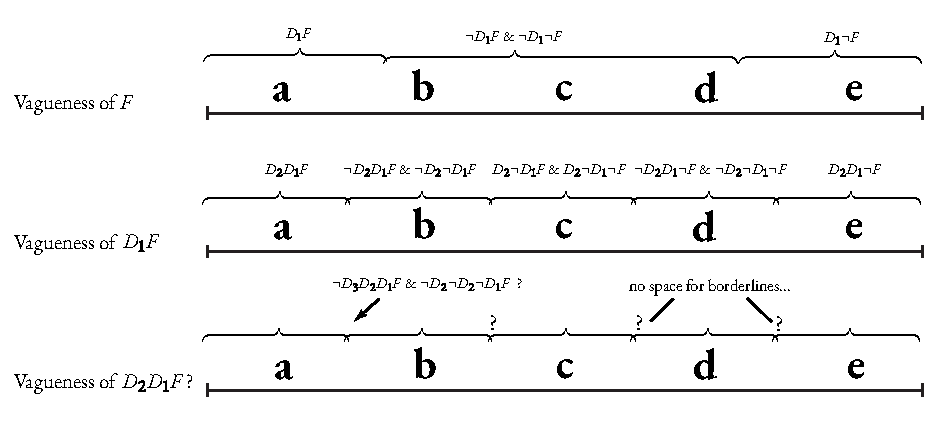
\includegraphics[width=0.925\textwidth]{papers/figures/2-2.pdf}
\end{center}
In conclusion, even though the rigid hierarchy in Keefe's structure
might be defended to some extent, her appeal to an infinite hierarchy is
fundamentally in conflict with the finite Sorites. There seems to be no
way to accommodate the problem without making strong alterations to the
model.

\section{Positive proposal --- dynamizing supervaluationism}

\subsection{Introducing dynamic supervaluationism}

I believe that Keefe's problems can be addressed by making the
structure's categories dynamic. My proposal is loosely based on
Hao--Cheng Fu's model.\footnote{Hao-Cheng Fu, ``Saving Supervaluationism
  from the Challenge of Higher--Order Vagueness Argument,'' in
  \emph{Philosophical Logic: Current Trends in Asia} (2017), 147-152.} Fu rejects Keefe's
claim that admissibility is vague and instead claims that, when
considering a vague predicate, we are using a well--defined set of
precisifications (p--sets). Keefe might argue this counterintuitive since
we do not know what is admissible. However, this knowledge is
unnecessary: the p--set is created when cases are categorized as true,
false, or borderline at time \(t_{1}\). For example, if 195cm and 190cm
are tall, 170cm is not, and 180cm is borderline, the p--set is implicitly
formed dividing cases into three groups, on my reading of Fu. Crucially,
we judge first; the p--set is constructed afterward. What follows in the
next paragraphs is my own development of the idea.

Fu applies the AGM theory\footnote{AGM refers to the
  Alchourrón--Gärdenfors--Makinson model of belief revision, which
  accounts for rational change in epistemic states represented as belief
  sets. The theory outlines how agents should expand, contract, or
  revise their beliefs while preserving logical coherence. For more
  detail, see Carlos E. Alchourrón, Peter Gärdenfors, and David
  Makinson, ``On the Logic of Theory Change: Partial Meet Contraction
  and Revision Functions,'' \emph{The Journal of Symbolic Logic} 50, no.
  2 (1985): 510--30.}
to give a complex account of the dynamics of p--sets; however, offers
little formalisation and does not explain how this idea could be applied
to the challenges of HOV\footnote{Fu, ``Saving Supervaluationism from
  the Challenge of Higher-Order Vagueness Argument,'' 149-152.}.
Moreover, Fu does not address the paradoxes of HOV, and it is difficult
to see how his account could solve them. In my view, we do not need such
an elaborate account. I propose that a p--set is dynamic solely in virtue
of changing when a case is judged inconsistently with it. For the sake
of clarity, consider the above example again. Imagine another person,
\textbf{x}, who is 168cm. You judge \textbf{x} as tall. This is clearly
inconsistent with your p--set at \(t_{1}\), since you judged 170cm as not
tall. Thus, adding \textbf{x} to the tall category updates the \(t_{1}\)
set to the \(t_{2}\) set with revised precisifications. This change
occurs by either (1) expanding (adding a precisification), (2)
contracting (removing one), or (3) both. Therefore, I retain the core
idea of dynamic p--sets and Fu's terminology but limit the scope of the
mechanism to a minimal principle: a p--set updates only when a judgment
is made that conflicts with it.

I will now attempt to formalise the above proposed working of p--sets,
which I will later apply to the challenges haunting supervaluationism.
Vagueness, on the dynamic view, remains semantic indecision. At the
first level, we follow Keefe's supervaluationism with a slight addition
of the temporal component. While Fu does not offer a formalisation of
his view in the spirit of Keefe's system with D operators, the following
temporal framework develops my own way of modelling dynamic p--sets using
temporally indexed D operators.

More precisely, at any time, t, cases divide into
\(D_{t}F,D_{t}{\sim}F\), and \({{\sim}D}_{t}F\ \; \& \; {{\sim}D}_{t}{\sim}F\):
that is true, false, and borderline. However, unlike in Keefe's view,
HOV arises not from undecided admissibility of a precisification but
from the instability of precisifications. Suppose that you make some
categorisations at \(t_{1}\). According to the p-set that you just
formed; some arbitrary case is classified as \(D_{1}F\). Now suppose
that you consider the series again, but you are no longer sure about the
definiteness of your classification. Thus, your p--set is adjusted at
\(t_{2}\), and according to it, the case is borderline. Therefore, from
\(t_{2}\)'s perspective it was a borderline definite case at \(t_{1}\)
(\({{\sim}D_{2}D}_{1}F\)).

In general, when considering a borderline case after categorisation at
\emph{t}, tolerance ensures a mis--categorisation. To see this, remember
that the supervaluation technique divides cases sharply into true,
false, and borderline. However, tolerance guarantees that when viewing
two neighbouring cases, we will not be able to tell the difference.
Therefore, there is a clear tension; we divided sharply, enabling a
border pair where, for instance, one member is true and another
borderline. However, since we cannot distinguish between neighbouring
cases, they must be categorised equally. That means that one of the
cases had to be categorised mistakenly and thus, the p--set must be
revised to maintain consistency in our judgments. When we reconsider the
series at \(t_{2}\), the earlier categorisations from \(t_{1}\) turn out
to be indefinite, as case memberships shift.

\subsection{Applying dynamic supervaluationism}

Having formalised the view, I will now apply it to the challenges of
HOV, starting with Williamson's $D^*$ argument. To attack the dynamic
approach, $D^*$ could be restated as the conjunction `DA at \(t_{1}\) \& DA
at \(t_{2}\) \& DA at \(t_{3}\) \& \ldots{} \& DA at \(t_{n}\)'. As
discussed in section 3, the $D^*$ argument establishes that, if $D^*$ is not
shown to be vague, then the cases where $D^*$ is true and the cases where
$D^*$ is false will both be ultimately definite. Hence, there will be no
borderline cases between $D^*$ categories, which provides a sharp boundary.
This contradicts the foundational supervaluationist claim that there are
no sharp boundaries. However, this argument loses its force under the
dynamic view. The dynamic framework allows us to easily account for the
vagueness of $D^*$. Just as in the case of any D, we need to progress in
time to express $D^*$'s vagueness. Thus, while $D^*$ may initially appear to
be non--vague, this is because we need to move to $t + 1$ to realize its
vagueness.

Secondly, Keefe's view faced concerns about rigid hierarchies, but the
dynamic approach eliminates these. When two speakers disagree over a
case's definiteness, neither statement must be `prior'. They are simply
speaking from different p--sets that underwent different evolutions.
There is no rigid hierarchy of metalanguages since each discusses
categorizations in another metalanguage, and no pair can be clearly
ranked as `prior'.

This lack of priority arises because it would be impossible to assign it
to any particular metalanguage. Surely, the metalanguage at $t+1$
must be a metalanguage of the metalanguage at $t$, since it is able
to express facts about $t$. Therefore, it is more `privileged' in
this sense. However, suppose that the p--sets evolve over time such that,
when moving from $t+1$ to $t+2$, we go back to the original
p--set from $t$. Then, the $t$ and $t+2$ metalanguages
gain their truth conditions from the same p--set. Therefore, in a sense,
the t metalanguage becomes `prior' to the $t+1$ metalanguage. This
would undermine the strict, unidirectional Tarskian hierarchy.

One could further argue that we could suppose a scenario in which two
identical people, A and B, undergo identical p--set evolutions. However,
A's evolution stops at \emph{t} and B's evolution stops at \emph{t}+1.
On the one hand, we might be tempted to assign priority to B's
statements, which would be counter--intuitive on the natural language
objection. However, there is no reason to suppose that A's evolution
should go the same way; she might consider a different part of the
Sorites spectrum. Therefore, although the metalanguages are in some
sense hierarchical, none has a clear priority in determining the truth
of one classification over another. Thus, the objections, such as the
ones made by Kripke, do not apply here.

Thirdly, the dynamic view can help tackle the finite series paradox,
which was a critical blow to Keefe's account. I will explain how it
could achieve this through an example. Consider a 5--element Sorites with
objects \textbf{a}, \textbf{b}, \textbf{c}, \textbf{d}, and \textbf{e}.
Suppose that Alfred's initial categorizations are:

\begin{center}
\begin{tabulary}{\textwidth}{RCL}
$D_1 F$ & = & $\{ \mathbf{a}, \mathbf{b} \}$ \\
${\sim}D_1 F \ \& \ {\sim}D_1{\sim}F$ & = & $\{ \mathbf{c} \}$ \\
$D_{1}{\sim}F$ & = & $\{ \mathbf{d}, \mathbf{e}\}$ \\
\end{tabulary}
\end{center}
Alfred considers the pair \textbf{b} and \textbf{c} again. He realizes
that he cannot tell the difference, concluding that \textbf{b} is also
borderline. He adjusts his p--set accordingly, forming a new \(t_{2}\)
p-set.

\begin{center}
\begin{tabulary}{\textwidth}{RCL}
$D_2 F$ & = & $\{ \mathbf{a} \}$ \\
${\sim} D_2 F \ \& \ {\sim}D_2 {\sim}F$ & = & $\{ \mathbf{b}, \mathbf{c} \}$ \\
$D_2 {\sim}F$ & = & $\{ \mathbf{d}, \mathbf{e} \}$
\end{tabulary}
\end{center}

\begin{center}
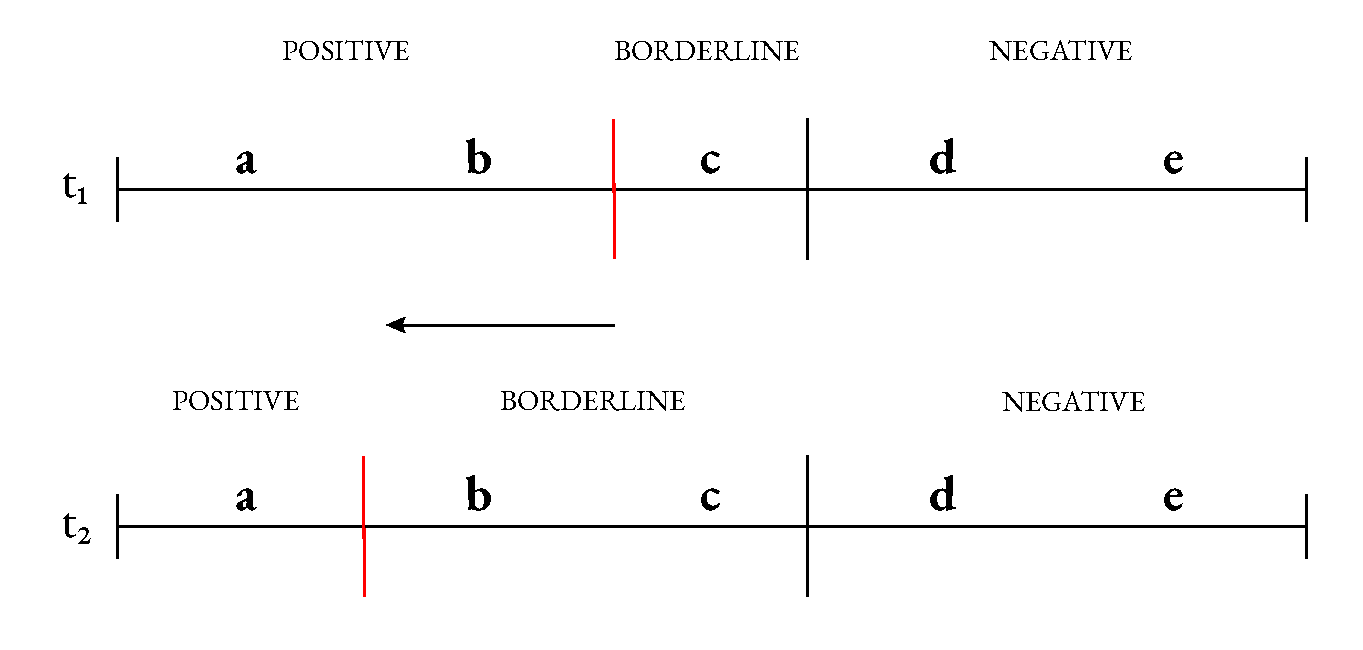
\includegraphics[width=4.50937in,height=2.12793in]{papers/figures/2-3.pdf}
 \end{center}
The $t_{1}$ division, from the perspective of $t_{2}$ becomes:

\begin{center}
\begin{tabulary}{\textwidth}{RCL}
$D_2 D_1 F$ & = & $\{ \mathbf{a} \}$ \\
${\sim} D_2 D_1 F \ \& \ {\sim}D_{2}{{\sim}D}_{1}F$ & = & $\{ \mathbf{b} \}$ \\
$D_{2}{\sim}D_{1}F\ \&\ D_{2}{\sim}D_{1}{\sim}F $ & = & $\{ \mathbf{c} \}$
\end{tabulary}
\end{center}

\begin{center}
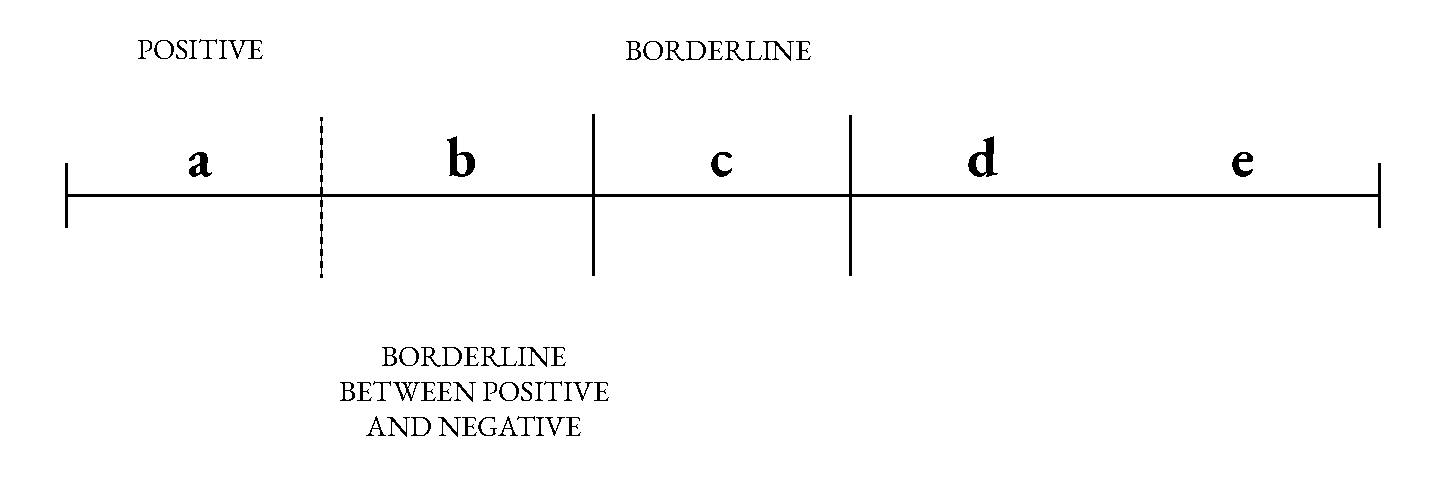
\includegraphics[width=0.77\textwidth]{papers/figures/2-4.pdf}
\end{center}
Hence, in this part of the series, the vagueness of \(D_{1}\) is fully
accounted for since all $D_{1}$ categories have borderline cases.

Now suppose that at time $t_{3}$, he looks at the pair $\mathbf{a}$ and
$\mathbf{b}$. Since he cannot tell the difference, he decides that b is
also a definite case, adjusting the p--set again.

\begin{center}
\begin{tabulary}{\textwidth}{RCL}
$D_3 F$ & = & $\{ \mathbf{a}, \mathbf{b} \}$ \\
${\sim} D_3F \ \& \ {\sim}D_{3}{\sim}F$ & = & $\{ \mathbf{c} \}$ \\
$D_{3}{\sim} F $ & = & $\{ \mathbf{d}, \mathbf{e} \}$
\end{tabulary}
\end{center}

\begin{center}
    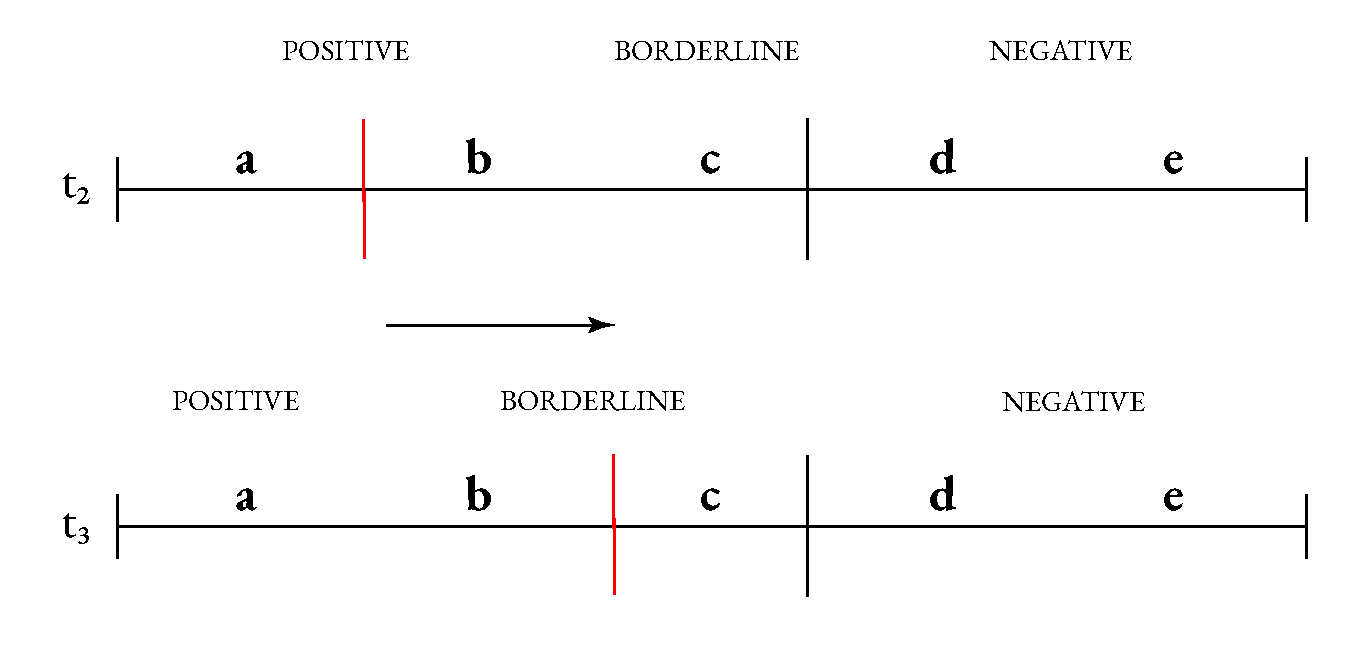
\includegraphics[width=4.46286in,height=2.2071in]{papers/figures/2-5.pdf}
  \end{center}
Since $\mathbf{b}$ changed its category membership, from the perspective
of \(t_{3}\), $\mathbf{b}$ was not a definite borderline case at
\(t_{2}\). Thus, the \(t_{2}\) division, from the \(t_{3}\) perspective,
is:

\begin{center}
\begin{tabulary}{\textwidth}{RCL}
$D_3 D_2 F$ & = & $\{ \mathbf{a} \}$ \\
${\sim}D_3 D_3 F \ \& \ {\sim}D_2 {\sim}D_2 F$ & = & $\{ \mathbf{b} \}$ \\
$D_3 {\sim}D_2 F \ \& \ D_3 {\sim}D_2 {\sim}F$ & = & $\{ \mathbf{c} \}$
\end{tabulary}
\end{center}

\begin{center}
    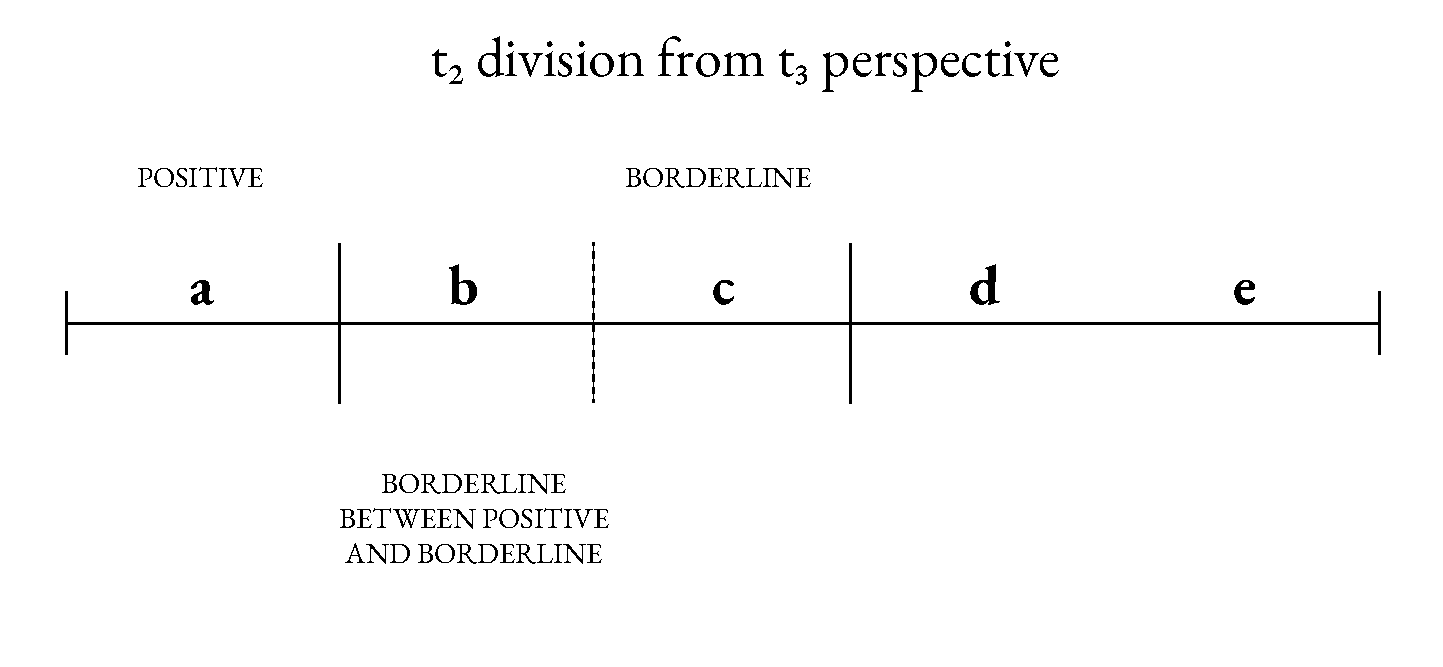
\includegraphics[width=0.77\textwidth]{papers/figures/2-6.pdf}
  \end{center}
Thus, vagueness of \(D_{2}\) is accounted for.

In general, any bordering pair will exhibit change when reassessed.
Thus, any categorization at $t$ can prove indefinite at $t+1$.
In effect, you will never reach a point where there are more categories
than members in the series since the fluid categories will always be
filled. An object can fill different categories at different times. This
also does not mean that the \(t_{1}\) categories are definite at
\(t_{3}\), only that their vagueness cannot be expressed from the
\(t_{3}\) perspective.

\section{Addressing possible objections}

Dynamizing supervaluationism provides new methods to tackle the
paradoxes of HOV and other problems, for which standard
supervaluationism struggles to account. However, it also presents new
worries, which I will explore and sketch responses to in this section of
the essay.

\subsection{Fixed time worry}

The first possible objection to the view is that it breaks down when
time is fixed. This is because the account of HOV relies on shifty
p-sets, which in turn rely on the progress in time. More precisely, the
vagueness of some set of categories drawn in period $t$ can only be
expressed in period $t+1$. Thus, if we hold the time fixed, the
view breaks down: the categories drawn in period $t$ appear to be
sharply bounded, which contradicts the foundational claim that there are
no sharp boundaries.

Although this might seem like a critical blow to the view, there are two
possible lines of response. First, we could simply reject the inference
from our inability to express the vagueness of some order when time is
fixed, to the claim that there are sharp boundaries. After all, the fact
that we cannot express it does not imply that it does not exist. This,
however, demands further explanation of why we cannot express it. One
response is that at a certain time, we are just using a well--defined but
arbitrary set of precisifications. However, this division is surely
wrong; it is made under one of many sets of equally good
precisifications. Thus, there is no reason to believe that the term was
made precise---we just have not realized our mistake yet.

A second and more powerful response is to deny the possibility of fixing
time in this sense. This could supplement the above argument. Suppose
that the critic of the view wants to prove to us that there are sharp
boundaries. However, in order to show that there are sharp boundaries,
they would have to find them in the series. Suppose that you manage to
find the extension--switching pair. Even if you do this, you will
realize, per tolerance, that you cannot tell the difference between the
two cases. In effect, you must conclude that one of the cases was
falsely classified when you made the division in the previous period.
Thus, your p--set changes. Therefore, the very considering of the sharp
distinction would automatically progress us to $t+1$, ensuring that there
was no sharp boundary. In conclusion, the fixed time objection is not a
significant worry to the dynamic view.

\subsection{Collapse to contextualism worry}

There is a second and more dangerous worry: one could argue that the
supervaluationist aspect of the dynamic view seems unimportant. By this,
I mean the use of supervaluationist semantics and classification of
vagueness through indecision between precisifications. It is only
directly applied to resolve FOV, and one could argue that the relativity
of classifications over time, which accounts for HOV, could be equally
applied to FOV. In effect, the supervaluationist method would disappear.
If this argument is accepted, and if we further assume that the
functioning of p-sets is sufficiently similar to that of contexts, then
the dynamic view risks collapsing into a contextualist one. This could
have some benefits, such as the preservation of bivalence (which
contextualists keep) and making the view more parsimonious by unifying
the approaches to vagueness at different orders.

In what follows, I will defend the dynamic view from this objection. See
footnotes for background on contextualism\footnote{Contextualism rests
  on the claim that vagueness is a species of context-sensitivity. This
  roughly means that, in its application across different contextual
  circumstances, a vague term maintains a constant \textit{character} but
  shifts in \textit{content}. Therefore, vague terms function like
  indexical terms. The relationship of vagueness and indexicality is a
  contested matter for contextualists. Some hold that vague terms behave
  \textit{like} indexicals, while others claim they \textit{are} indexicals.
  However, this distinction is not directly relevant to the discussion,
  and the objections raised here apply equally to both views. Consider
  the word \textit{now}. It adheres to the same grammatical rules (i.e.,
  has the same \textit{character}) when uttered today and tomorrow.
  However, when said today, it picks out a different time than it does
  when used tomorrow (i.e., has different \textit{content}). Similarly, a
  vague predicate like \textit{tall} is used in the same way when applied
  to members of a group of pygmy peoples, as when applied to a group of
  Dutch people. However, it would pick out radically different people.
  In the first case, the extension of \textit{tall} likely includes some
  of the world's shortest people; in the second, some of the tallest.
  See Roy Sorensen, ``Vagueness,'' \textit{The Stanford Encyclopedia of
  Philosophy} (Winter 2023 Edition), ed. Edward N. Zalta and Uri
  Nodelman.}
and their solution to the Sorites.\footnote{Contextualists exploit this
  idea of unstable extensions over contexts to solve the Sorites by
  accusing it of equivocating different meanings of a vague term.
  Similarly to the supervaluationists, the contextualists target the
  inductive premise (2). The contextualist is committed to the claim of
  weak tolerance (WT), which states that when two members of a bordering
  pair are considered in the same context $C$, they will belong to the
  same extension. However, WT permits that when one member is considered
  in context $C$ and the other in $C^\prime$, then they might belong to a
  different extension. See Jonas Åkerman and Patrick Greenough, "Hold
  the Context Fixed---Vagueness Still Remains," in \textit{Relative
  Truth}, ed. Manuel García-Carpintero and Max Kölbel (Oxford University
  Press, 2010), 275--76.

  The WT explains why the inductive premise seems to hold. If we
  consider any pair in the series, we will conclude that both members
  belong to the same extension. But this is just because we are disposed
  to view them in the same context $C$. The contextualist says that, in
  fact, the context will gradually change across the series. This means
  that even if we classify neighbouring terms the same at first, this
  classification will not persist throughout the series. Thus, the
  inductive premise of the sorites, such as `if $\mathbf{n}$ is short, then $\mathbf{n}+1$ is short', fails since the meaning of `short' is not the same for every
  member $\mathbf{n}$. This is because, the shift of context $C$ into $C^\prime$,
  enables cases where `$\mathbf{n}$ is short' is true (in $C$) but `$\mathbf{n}+1$ is short' is false (in $C^\prime$). See J. Åkerman, "Contextualist Theories of Vagueness,"
  \textit{Philosophy Compass} 7 (2012): 470--75.}
The first point that I address is the idea that supervaluation is
obsolete. On this view, its role at the first level could be replaced by
the context--reminiscent p--sets. The intuitive idea is that, since shifty
p--sets account for HOV, why not apply them to FOV and get rid of
additional semantic claims and concessions altogether? However, this
intuition is misguided, since the supervaluationist solution to FOV is
required to make the shifty p--set account of HOV work. This is because
the first--order divisions allow for the p--sets to shift in the first
place. At the first stage, we implicitly categorize objects into
positive, negative, and borderline cases. These categories are directly
determined by the p--set, which sets out the supervaluationist truth
conditions (i.e., $DF$ iff true for all precisifications and so on). These
categorizations are provisional: they impose sharp boundaries where none
truly exist. This tension allows for future revisions of p--sets, and
thus for p--sets to shift. Hence, without supervaluation in the
beginning, the p--sets cannot shift. And if they cannot shift, they
cannot account for any order of vagueness.

A stronger claim could be made that the p-sets are entirely purposeless
if we do not allow for supervaluation. To see the point, imagine that
you have some set of precisifications of tall $\{>170\text{cm},
>180\text{cm}, >190\text{cm}\}$ and you use them to categorize a
group of people in the series. Without supervaluation, you end up with
six extensions, i.e., three positive and three negative extensions, one
per precisification. There are no borderline cases, since without
supervaluationist truth conditions---where borderlines are true under
some precisifications and false under others---such cases are not
defined. Since this is a key symptom of vagueness, as stressed in the
beginning, this result would require further explanation of why we think
there are borderlines at all.

An enemy of the view could argue that this response misses the point---vagueness did not fail to arise due to the absence of supervaluation,
but rather because the p--sets did not shift. After all, on the dynamic
account, it is the shiftiness of p--sets that allows for HOV. To address
this, let us suppose, for the sake of the argument, that the p-set can
somehow shift without supervaluation. Imagine, for instance, that the
p--set expands by incorporating an additional precisification to the set.
You now have eight extensions, yet still no explanation for either
first--order or higher-order vagueness. Thus, even with shifty p--sets,
the dynamic view cannot function without supervaluation, showing it to
be an essential, not merely supportive, component of the account.

Therefore, the case for the contextual collapse breaks down in the very
beginning. We simply cannot make the p-sets shifty without maintaining
the baseline supervaluationist aspects of the theory. If we cannot make
the p-sets shifty, they cannot resolve FOV, let alone HOV. Hence,
supervaluation is by no means obsolete. However, to strengthen the
defense, I will demonstrate that the next step needed for the
contextualist collapse fails. That is, I will show that p--sets and
contexts behave very differently.

Although they might appear similar, the former crucially relies on the
characterization of vagueness as semantic indecision, while the latter
depend on context sensitivity. We might express this difference by
saying that the p--sets are inward--oriented, while contexts are more
outward--oriented. This is because the former shifts due to our
indecision among several equally good precisifications at the initial
stage. This indecision prompts us to make mistakes, which we
subsequently correct by revising the p--set into another equally
acceptable p-set. Thus, the changes directly follow our judgments. By
contrast, shifts in contexts seem to have an effect on our judgments---contexts shift first, and judgments follow. Thus, the machinery appears
to be quite different.

One could even argue that shifty p-sets rest on a firmer theoretical
ground---their shiftiness is caused by our inconsistent judgments. On
the other hand, the contexts appear to shift arbitrarily. Thus, the
contextualist requires some external justification for this instability.
Additionally, the contextualist needs to show how contexts could become
shifty enough to prevent every instance of the Sorites. In other words,
enough shiftiness must be generated. I do not intend to digress further,
but the key takeaway is that despite their apparent similarities, p--sets
and contexts differ significantly. Thus, the threat of the `collapse'
does not seem to be so imminent.

As a final point to strengthen my argument, I will provisionally assume
that the dynamic approach could collapse into contextualism. Even in
such a scenario, there remain independent reasons to prefer the former
view over the latter. One significant reason is that contextualism
undermines some of our most basic approaches to reasoning. Contextualism
requires extensions of vague terms to be unstable, which is precisely
what enables it to defeat the Sorites. However, these shifty contexts
become deeply problematic when applied outside of the paradoxical
setting.

To see this, consider the following example. Saul and Jan are borderline
cases of tall. The former is 176.1cm, and the latter is 176cm. Suppose
you judge both of them to be tall. Now consider applying the following
instance of conjunction introduction:

\begin{center}
  $\cfrac{\text{Saul is tall} \hspace{2em} \text{Jan is tall}}
  {\text{Saul and Jan are tall}}  { \ \land  } \ \text{I} $
\end{center}
However, if the extension of the vague predicate \emph{tall} is
unstable, we can easily imagine a situation in which both premises are
individually true, yet the conclusion turns out false. This would happen
if the context shifted midway through the argument. Thus, although
context sensitivity is useful for solving the Sorites, it is dangerous
when applied to everyday reasoning. Specifically, how can contexts
remain sufficiently stable to ensure our logic does not fail even in
such simple cases?\footnote{J. Åkerman, "Contextualist Theories of
  Vagueness," \emph{Philosophy Compass} 7 (2012): 475--76,
  \href{https://doi.org/10.1111/j.1747-9991.2012.00495.x}.}

In contrast, dynamic supervaluationism does not provoke such worries.
Under supervaluationism, the rule of a conjunction introduction always
preserves validity. To illustrate, consider a p--set representing
precisifications for \emph{tall}: \{\textgreater170, \textgreater175,
\textgreater176\}. First two precisifications make both premises true
and the conclusion true as well. The third precisification makes one of
the premises true, the other false, and the conclusion false. This will
work for any possible precisification. Consequently, it applies to every
p-set.\footnote{This follows the exact same reasoning as that applied to
  the failure of the inductive premise or the truth of the law of
  excluded middle discussed in more detail at the beginning of the
  essay.}

One might argue that, similarly to a shifting context, the p--set could
shift over the course of an argument. For example, we might initially
classify both premises as true (e.g., using the set \{\textgreater170,
\textgreater175\}, but later we classify the conclusion as false (e.g.,
shifting to the set \{\textgreater177, \textgreater180\}). However, this
objection reflects a misunderstanding of supervaluationist semantics,
since arguments must always be evaluated relative to a single p--set. If
we shifted the p--set to the second one, both premises would become false
along with the conclusion. Therefore, the validity of conjunction
introduction would remain intact.

Why is this strategy not available to the contextualist? The
contextualist could simply deny that contexts can shift in such ways,
insisting instead that we always evaluate the premises and the
conclusion within a single context. However, this directly contradicts
the contextualist's equivocation strategy to the Sorites paradox. That
is, the strategy according to which bordering cases may differ in truth
value because their evaluation contexts differ. Hence the contextualists
need contexts to shift. In effect, they cannot deny that the above
scenario is possible. Instead, their strongest response would likely be
to argue that such cases rarely happen.

I do not intend to argue that supervaluationism, or its dynamic version,
is superior to contextualism. Such a claim is clearly beyond the scope
of this essay and perhaps beyond the scope of any single essay. Rather,
my point is simply that there are independent reasons to prefer the
dynamic view over contextualism. Therefore, the claim that contextualism
explains everything that the dynamic view explains---but more simply,
and thus more parsimoniously---is clearly not accurate.

Taking stock of these considerations, the collapse argument fails not
only at its initial stage but also on all subsequent fronts. Dynamic
supervaluationism is by no means contextualism in disguise; rather it is
its own theory, deeply grounded in Keefe's original supervaluationist
framework.

\section{Conclusion}

While Keefe's supervaluationism remains an attractive account of
vagueness, it ultimately struggles to account for higher--order
vagueness. Her adoption of a rigid, Tarskian infinite hierarchy may
block Williamson's $D^*$ argument, but at the cost of disconnecting the
theory from natural language. Even if, as I briefly explored, she could
respond to these problems, adopting an infinite metalanguage hierarchy
still leaves Keefe subject to a seemingly unresolvable finite series
paradox. I argued that Keefe's account could be dynamized by
incorporating ideas from Fu, thereby resolving the finite series paradox
and avoiding issues associated with a rigid hierarchy. Yet, the dynamic
model itself introduces new difficulties, notably the `fixed time' and
`collapse to contextualism' problems. To defend the view, I briefly
outlined potential replies to these issues, showing that they are not
fatal. Dynamizing supervaluationism may not resolve all problems, but it
is a promising development of the supervaluationist theory and would be
worth elaborating on and defending in future enquiries.

\subsection*{Appendix}

\subsubsection*{Why must Keefe deny the S4 and S5 principles?}

\begin{enumerate}
\def\labelenumi{(\arabic{enumi})}
\item The S5 principle: If ${\sim}DF$ then $D{\sim}DF$.
\item The S4 principle: If $DF$ then $DDF$. 
\end{enumerate}
Suppose that (1) and (2) hold and that we have the first--order
classification:
\begin{enumerate}
  \def\labelenumi{(\roman{enumi})}
\item{$DF$ for definite positive cases.}
\item{${\sim}DF \ \& \ {\sim}D{\sim}F$ for borderline cases.}
  \item{$D{\sim}F$ for negative cases.}
  \end{enumerate}

If (1) holds, it implies that at the second level, $DF$ and
$D{\sim}F$ transform into $DDF$ and $DD{\sim}F$ (see proofs a and
b). That is, the definite positive and definite negative case is
definitely definite positive and definitely definite negative,
subsequently. If (2) holds, it implies ${\sim}DF\ \&\  {\sim}D {\sim}F$
${\sim}DF \ \& \ {\sim}D{\sim}F$ transforms into $D{\sim}DF \ \& \ D{\sim}D{\sim}F$ (see proof c). That is,
the borderline case is definitely a borderline case. However,
second--order vagueness would require two more categories---the
borderline between positive and borderline
(${\sim}DDF \ \& \ {\sim}D{\sim}DF$) and the borderline between borderline
and negative (${\sim}DD{\sim}F \ \& \ {\sim}D{\sim}D{\sim}F$). As a result,
sharp boundaries are drawn between the three categories since there are
no cases between them.

% \includegraphics[width=3.125in,height=1in]{media/image7.png}

%\includegraphics[width=2.87025in,height=0.94231in]{media/image8.png}
\bigskip
\noindent
\begin{minipage}[t]{0.48\textwidth}
    \noindent \textbf{Proof a:} \\
    \begin{center}
    $\cfrac{
        DF \hspace{2em} DF \rightarrow DDF
    }{DDF} {\ \rightarrow \hspace{-0.25em} E}$
    \end{center}
\end{minipage}
\begin{minipage}[t]{0.48\textwidth}
  \noindent \textbf{Proof a:} \\
    \begin{center}
    $\cfrac{
        D \neg F \hspace{2em} D\neg F \rightarrow DD \neg F
    }{DD\neg F} {\ \rightarrow \hspace{-0.25em} E}$
    \end{center}
  \end{minipage}
\bigskip

\noindent \textbf{Proof c:}
  \begin{center}
    $\cfrac{
        \cfrac{
        \begin{array}{c}
        \\
        \neg DF \rightarrow D \neg DF
        \end{array}
        \cfrac{
            \neg DF \neg D \neg F
        }{\neg DF} {\land E}
        }{D \neg DF} {\ \rightarrow \hspace{-0.25em}E} \hspace{1em}
        \cfrac{
            \cfrac{\neg DF \land \neg D \neg F}{\neg D \neg F} {\land E} \hspace{1em}
            \begin{array}{c}
            \\
            \neg D \neg F \rightarrow D \neg D \neg F
            \end{array}
        }{D \neg D \neg F}{\ \rightarrow \hspace{-0.25em}E}
    }{D\neg D F \land D\neg D\neg F} {\land I}$
    \end{center}

%\includegraphics[width=6.26806in,height=1.61181in]{media/image9.png}

\refsection
  
\begin{hangparas}{\hangingindent}{1}
Åkerman, Jonas. "Contextualist Theories of Vagueness." \emph{Philosophy
Compass} 7 (2012): 470--80.

Åkerman, Jonas, and Patrick Greenough. ``Hold the Context
Fixed---Vagueness Still Remains.'' In \emph{Relative Truth}, edited by
Manuel García-Carpintero and Max Kölbel, 275--288. Oxford: Oxford
University Press, 2010.

Alchourrón, Carlos E., Peter Gärdenfors, and David Makinson. ``On the
Logic of Theory Change: Partial Meet Contraction and Revision
Functions.'' \emph{The Journal of Symbolic Logic} 50, no. 2 (1985):
510--30. https://doi.org/10.2307/2274239.

Bobzien, Susanne. "In Defense of True Higher-Order Vagueness."
\emph{Synthese} 199, no. 3--4 (2021): 10197--10229.

Fine, Kit. \emph{Vagueness: A Global Approach.} Rutgers Lectures in
Philosophy Series. New York: Oxford Academic, 2020. Online edition, May
21, 2020. \url{https://doi.org/10.1093/oso/9780197514955.001.0001}.
Accessed November 15, 2024.

Fu, Hao-Cheng. ``Saving Supervaluationism from the Challenge of
Higher-Order Vagueness Argument.'' In \emph{Philosophical Logic: Current
Trends in Asia}, 139--52. 2017.

Greenough, Patrick. ``Higher-Order Vagueness.'' \emph{Proceedings of the
Aristotelian Society, Supplementary Volumes} 79 (2005): 167--90.
\url{http://www.jstor.org/stable/4106939}.

Hyde, Dominic. "Why Higher-Order Vagueness Is a Pseudo-Problem."
\emph{Mind} 103, no. 409 (1994): 35--41.

Keefe, Rosanna. \emph{Theories of Vagueness.} Cambridge: Cambridge
University Press, 2000.

Keefe, Rosanna. ``Vagueness: Supervaluationism.'' \emph{Philosophy
Compass} 3, no. 2 (2008): 315--24.

Kripke, Saul. ``Outline of a Theory of Truth.'' \emph{The Journal of
Philosophy} 72, no. 19 (1975): 690--716.
\url{https://www.jstor.org/stable/2024634}. Accessed November 30, 2024.

MIT OpenCourseWare. \emph{Session 11: Mathematics for Computer Science.}
\emph{6.042J: Mathematics for Computer Science, Spring 2015.}
Massachusetts Institute of Technology, 2015. Accessed December 8, 2024.

Sainsbury, Mark. ``Concepts without Boundaries.'' Chapter three of
\emph{Departing From Frege}. London: Routledge, 1990.

Sorensen, Roy. ``Vagueness.'' \emph{The Stanford Encyclopedia of
Philosophy} (Winter 2023 Edition), edited by Edward N. Zalta and Uri
Nodelman.
\href{https://plato.stanford.edu/archives/win2023/entries/vagueness/}.

Williamson, Timothy. \emph{Vagueness.} London: Routledge, 1994.
\end{hangparas}
%%% Local Variables:
%%% mode: LaTeX
%%% TeX-master: "../main"
%%% End:
